\imtnechapitre{Synthèse des travaux réalisés}
\setcounter{section}{0}
\section{Mission principale}
Ma première mission a été de mettre en place du monitoring sur un résolveur interne à l’afnic.

Pour cela, j’ai commencé par installer un résolveur sur un vps en suivant un guide présent sur le gitlab interne afin de bien comprendre comment les différents programmes qui composent un résolveur fonctionnent et interagissent entre eux.

Ensuite j’ai essayé plusieurs méthodes pour récupérer les données intéressantes, notamment les données de consommation électrique du serveur qui ne sont évidentes à récupérer.
Une solution simple mais très peu précise est de récupérer le uTime (le nombre de cycles du processeur utilisés) des différents programmes afin de voir leur évolution.

Une deuxième solution que j’ai ensuite trouvée est l’utilisation d’un outil appelé Scaphandre qui permet de récupérer directement la consommation électrique du processeur en temps réel. Cet outil bien que très pratique est encore en développement et possède de nombreuses limitations, premièrement il ne peut pas récupérer les données de consommation des cartes graphiques (pas un problème dans notre cas) et il ne marche dans les machines virtuelles (VM) que s’il est aussi installé sur la machine physique et configuré manuellement pour chaque machine virtuelle ce qui n’est pas le cas pour les fournisseurs cloud tels que OVH, Azure (Microsoft), AWS (Amazon) et Google Cloud.

Après avoir tester plusieurs méthodes, j’ai décidé de récupérer les données grâce a Prometheus car l’organisation possédait déjà une instance Prometheus et parce que tous les programmes utilisés peuvent exposer leurs statistiques dans un format compatible.
Une fois l’architecture du système conçue, j’ai dû apprendre le fonctionnement des dockers afin de pouvoir intégrer les nouveaux outils ainsi que les changements de configuration nécessaires a leur fonctionnement, a la récupération de statistique et a l’activation des interfaces Prometheus.

Après plusieurs cycles de modifications afin de que tout marche comme prévu à l’intérieur des différents dockers.

En parallèle, j’ai demandé l’ouverture des flux entre le serveur Prometheus et le résolveur (sur les différents ports donnant accès aux interfaces Prometheus).

Une fois tous les flux fonctionnels, j’ai créé un nouveau dashboard (tableau de bord) dans le grafana interne (déjà relié au serveur Prometheus) et fait des graphiques avec les informations intéressantes :

\begin{itemize}
    \item La consommation totale du serveur
    \item La consommation des différents processus du résolveur (il y a d’autres services tournant sur le même serveur)
    \item Le nombre de requêtes en Cache/Pas en Cache par seconde
    \item Le nombre de requête de chaque type (DoH,DoT,Dns) par seconde
\end{itemize}

\begin{figure}[htbp]
  \centering
  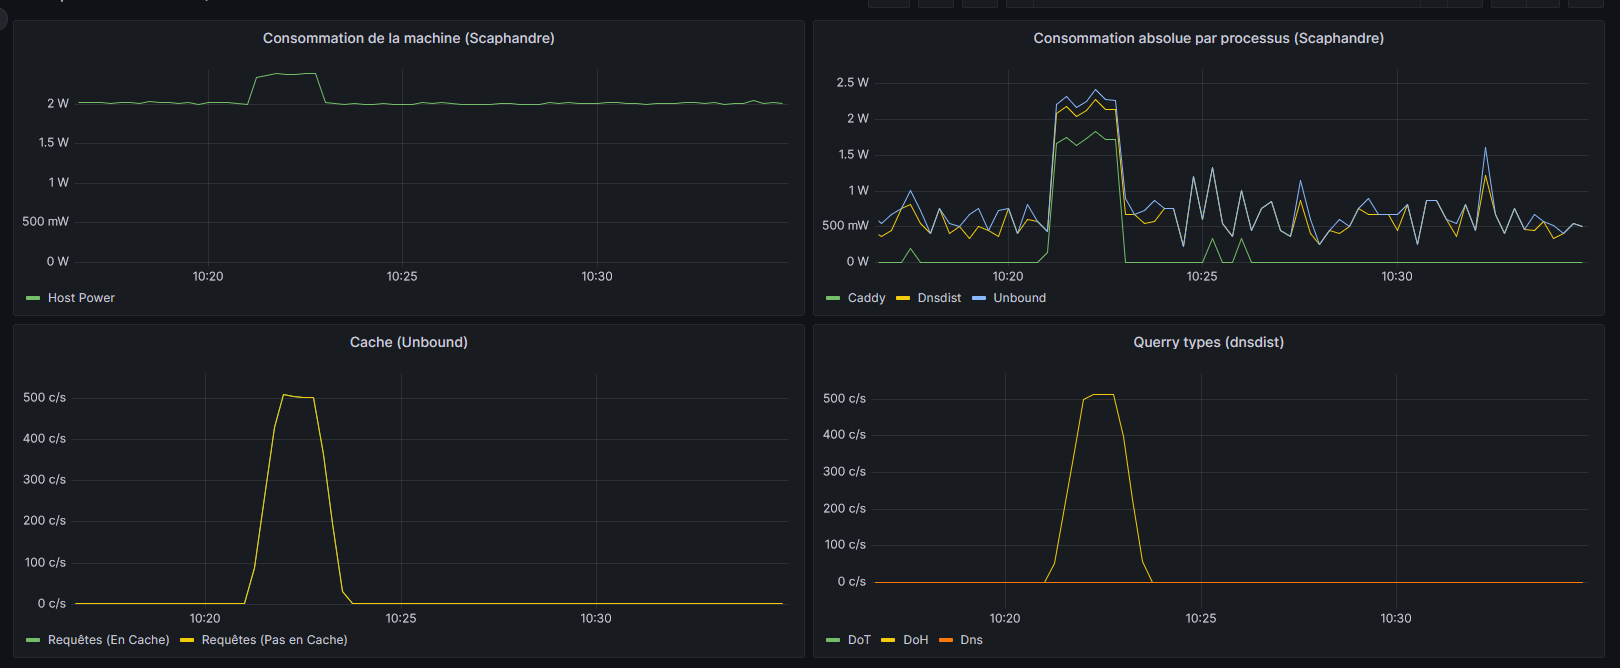
\includegraphics[width=\textwidth]{paper/figures/grafanaDNS.png}
  \caption{Tableau de Bord Grafana}
  \label{fig:grafanaDNS}
\end{figure}


\section{Outil de génération de requêtes DoH}
A côté de ça, j’ai développé un simple outil web (page en pur html+js, aucune interaction côté serveur) afin de pouvoir tester le résolveur DoH sous charge.
Il permet de rentrer l’adresse du résolveur, les types d’enregistrement DNS a demander, et le délai entre chaque requête. J’y ait plus tard ajouté la possibilité d’importer une liste de noms de domaines via csv afin de remplacer celle par défaut (Top 1000 Alexa) 

\begin{figure}[htbp]
  \centering
  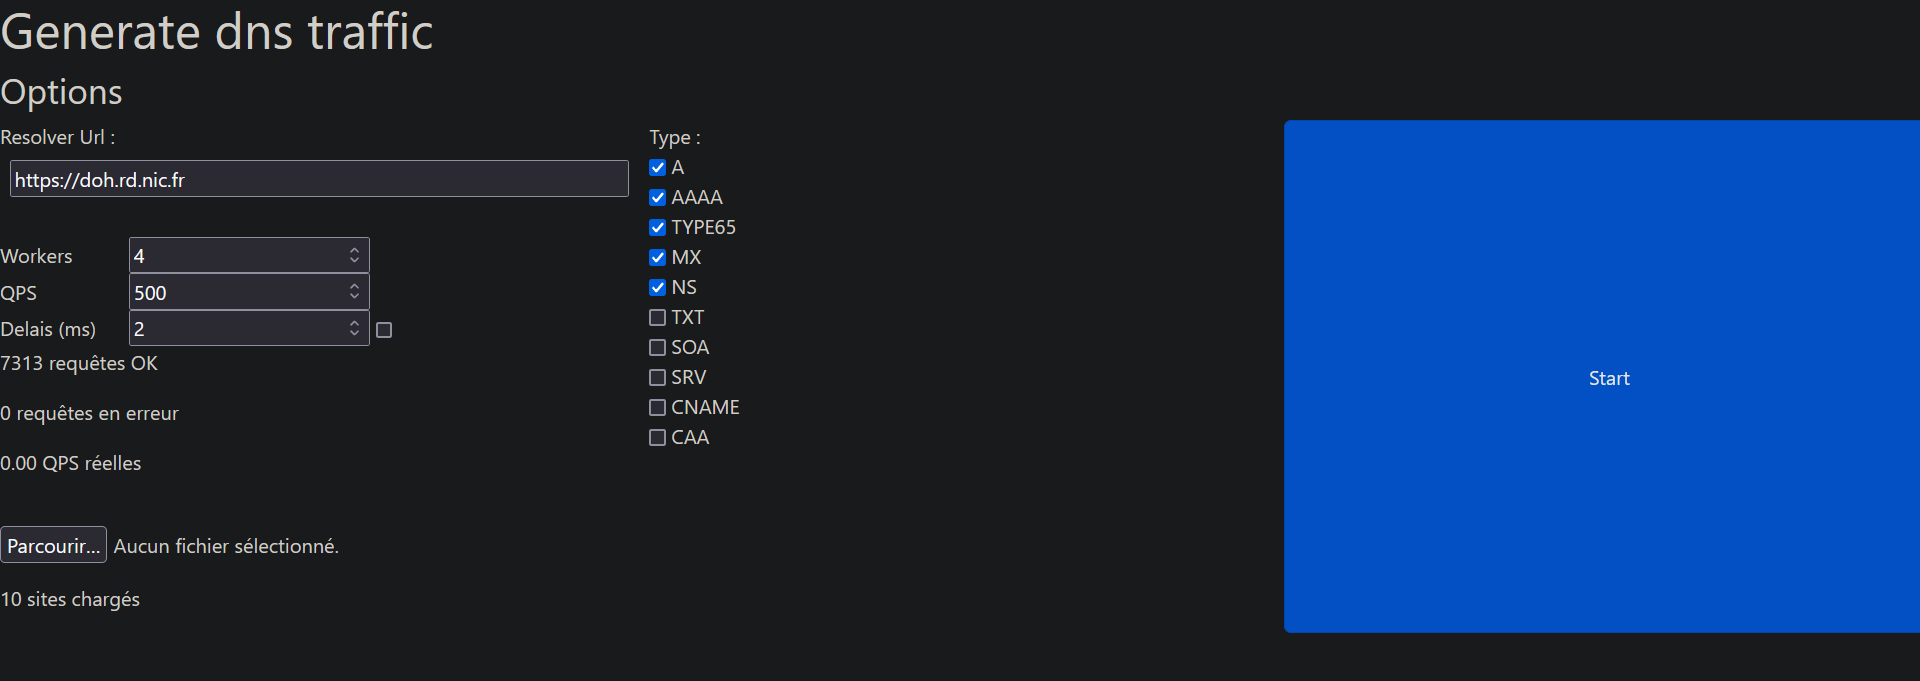
\includegraphics[width=\textwidth]{paper/figures/outilDoh.png}
  \caption{Visuel de l'outil de génération de requêtes DoH}
  \label{fig:outilDoh}
\end{figure}


J’ai ensuite créé un « virtual host » sur le serveur web interne et ajouté l’enregistrement correspondant dans le résolveur dns interne afin de pouvoir y accéder facilement depuis le réseau de l’organisation.

 
\section{Interface entre Wattmètres et Grafana}

Une autre de mes missions a été d’interfacer les Wattmètres (APCs) installés dans les baies de serveurs dans les deux principaux datacenters (TH3 et Marseille) utilisés pour la production (principalement \gls{anycast} DNS \todo{vrai ?)}) avec le système de monitoring central (Prometheus \verb|&| Grafana) afin de remplacer Observium qui bien qu'ayant une intégration native avec le protocole SNMP (Simple Network Management Protocol) utilisé pour communiquer avec les APCs n'est pas du tout ergonomique et demande de nombreux clics pour récupérer les informations nécessaires sans possibilités de les centraliser.

Le principal problème avec le fait d'interfacer des outils snmp avec prometheus est que Prometheus "\Gls{scrape}" les données, c'est a dire qu'il vas chercher "Des données" toutes les x secondes/minutes et stocke ce qu'il trouve alors que pour récupérer des données via le protocole SNMP, il faut demander les données que l'on souhaite. Il y a aussi le fait que les données renvoyés par SNMP ne sont pas dans un format compatible avec SNMP.

Pour résoudre ce problème, j'ai trouvé un outil appelé snmp\_exporter qui permet de faire la liaison entre les deux. Quand il reçois une requête de Prometheus (qui contient l'adresse de l'appareil SNMP cible ainsi que le nom du "Module" a utiliser), il vas chercher dans sa config le Module correspondant qui indique quelles sont les données souhaités puis vas les demander via SNMP a l'appareil, les met en forme afin qu'elles soient lisibles par Prometheus et finalement renvois cette réponse avec les données correctement formatés a Prometheus.

\todo{lien vers la doc}

\begin{figure}[htbp]
  \centering
  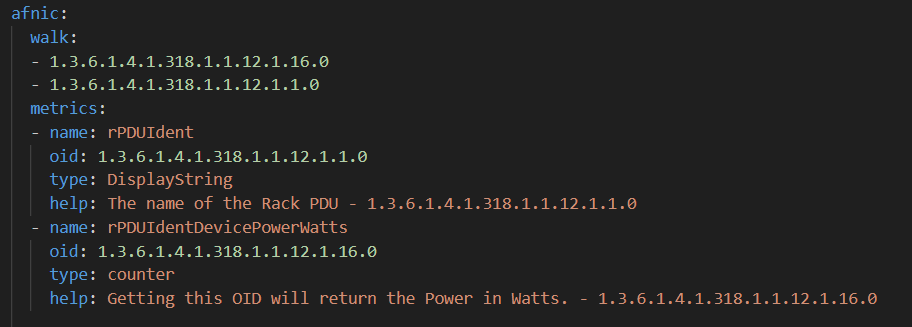
\includegraphics[width=\textwidth]{paper/figures/exempleConfigSNMP.png}
  \caption{Exemple de fichier de configuration de snmp\_exporter}
  \label{fig:exempleConfigSNMP}
\end{figure}

\todo{Rajouter nomad ?}

Une fois tout cela fait, on peut directement afficher toutes ces données sur Grafana :
\begin{figure}[htbp]
  \centering
  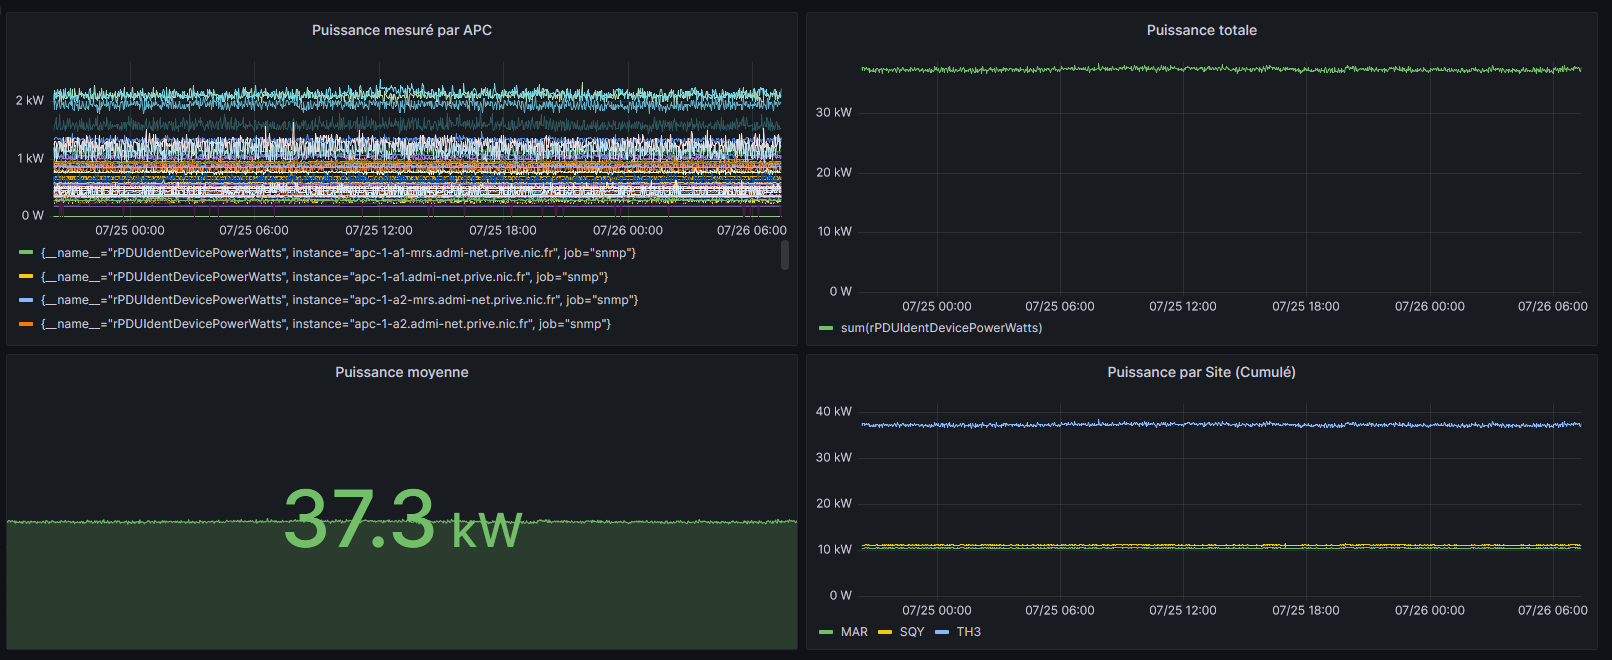
\includegraphics[width=\textwidth]{paper/figures/GrafanaAPC.png}
  \caption{Tableau de Bord Grafana APCs}
  \label{fig:GrafanaAPC}
\end{figure}

\section{Analyse des données récupérés}

Avant de commencer a analyser les données récupérés, il est important de préciser ce qu'elles représentent.
Ici nous allons uniquement étudier les données de consommation de serveurs (la machine physique) en corélation avec le nombre de requêtes dns traités.
Toutes les autres sources de consommation tels que les routeurs, firewall ou tout autre intermédiaire par lesquels passent les requêtes dns ne sont pas pris en compte.

Pour le résolveur, nous avons utilisé un serveur Bare Metal (gamme où la totalité d'un serveur est loué et non seulement un machine virtuelle) Rise-APAC-1 \todo{a vérifier, correspond a part pour modèle CPU, probablement plus disponible} avec ces caractéristiques :
\begin{itemize}
    \item Intel Xeon E3-1270v6 (4 coeurs/8 threads, 3.8GHz)
    \item 32 Go de RAM ECC DDR4
    \item SSD NVMe
    \item 500Mb/s de Bande passante
\end{itemize}

Cette configuration est bien au delà de ce qui est nécessaire pour un résolveur dns de faible ampleur cependant c'est une des plus basses qui correspondait a nos besoins :
\begin{itemize}
    \item Bare Metal du fait des limitations de Scaphandre
    \item Bande passante conséquente afin que ça ne soit pas un facteur limitant lors des mesures
\end{itemize}


\subsection{Résolveur}

\begin{figure}[ht]
  \noindent
  \begin{minipage}{.65\textwidth}
Pour ce qui est du résolveur, on remarque deux parties spécifiques :

Pour des volumes relativement faibles, la consommation électrique du serveur est constante et ne diffère pas de la consommation de référence (quand le serveur ne fait rien).

Pour des volumes plus élevés (plusieurs centaines voir milliers de requêtes par seconde), la consommation est plus ou moins lié de façon linéaire au nombre de requêtes reçues par seconde.

Ceci est lié au cpu (donc les données dépendent fortement du modèle de processeur utilisé) dont la consommation n'est pas linéairement lié a son utilisation. 
  \end{minipage}
  \hfill
  \begin{minipage}{.30\textwidth}
    \centering
      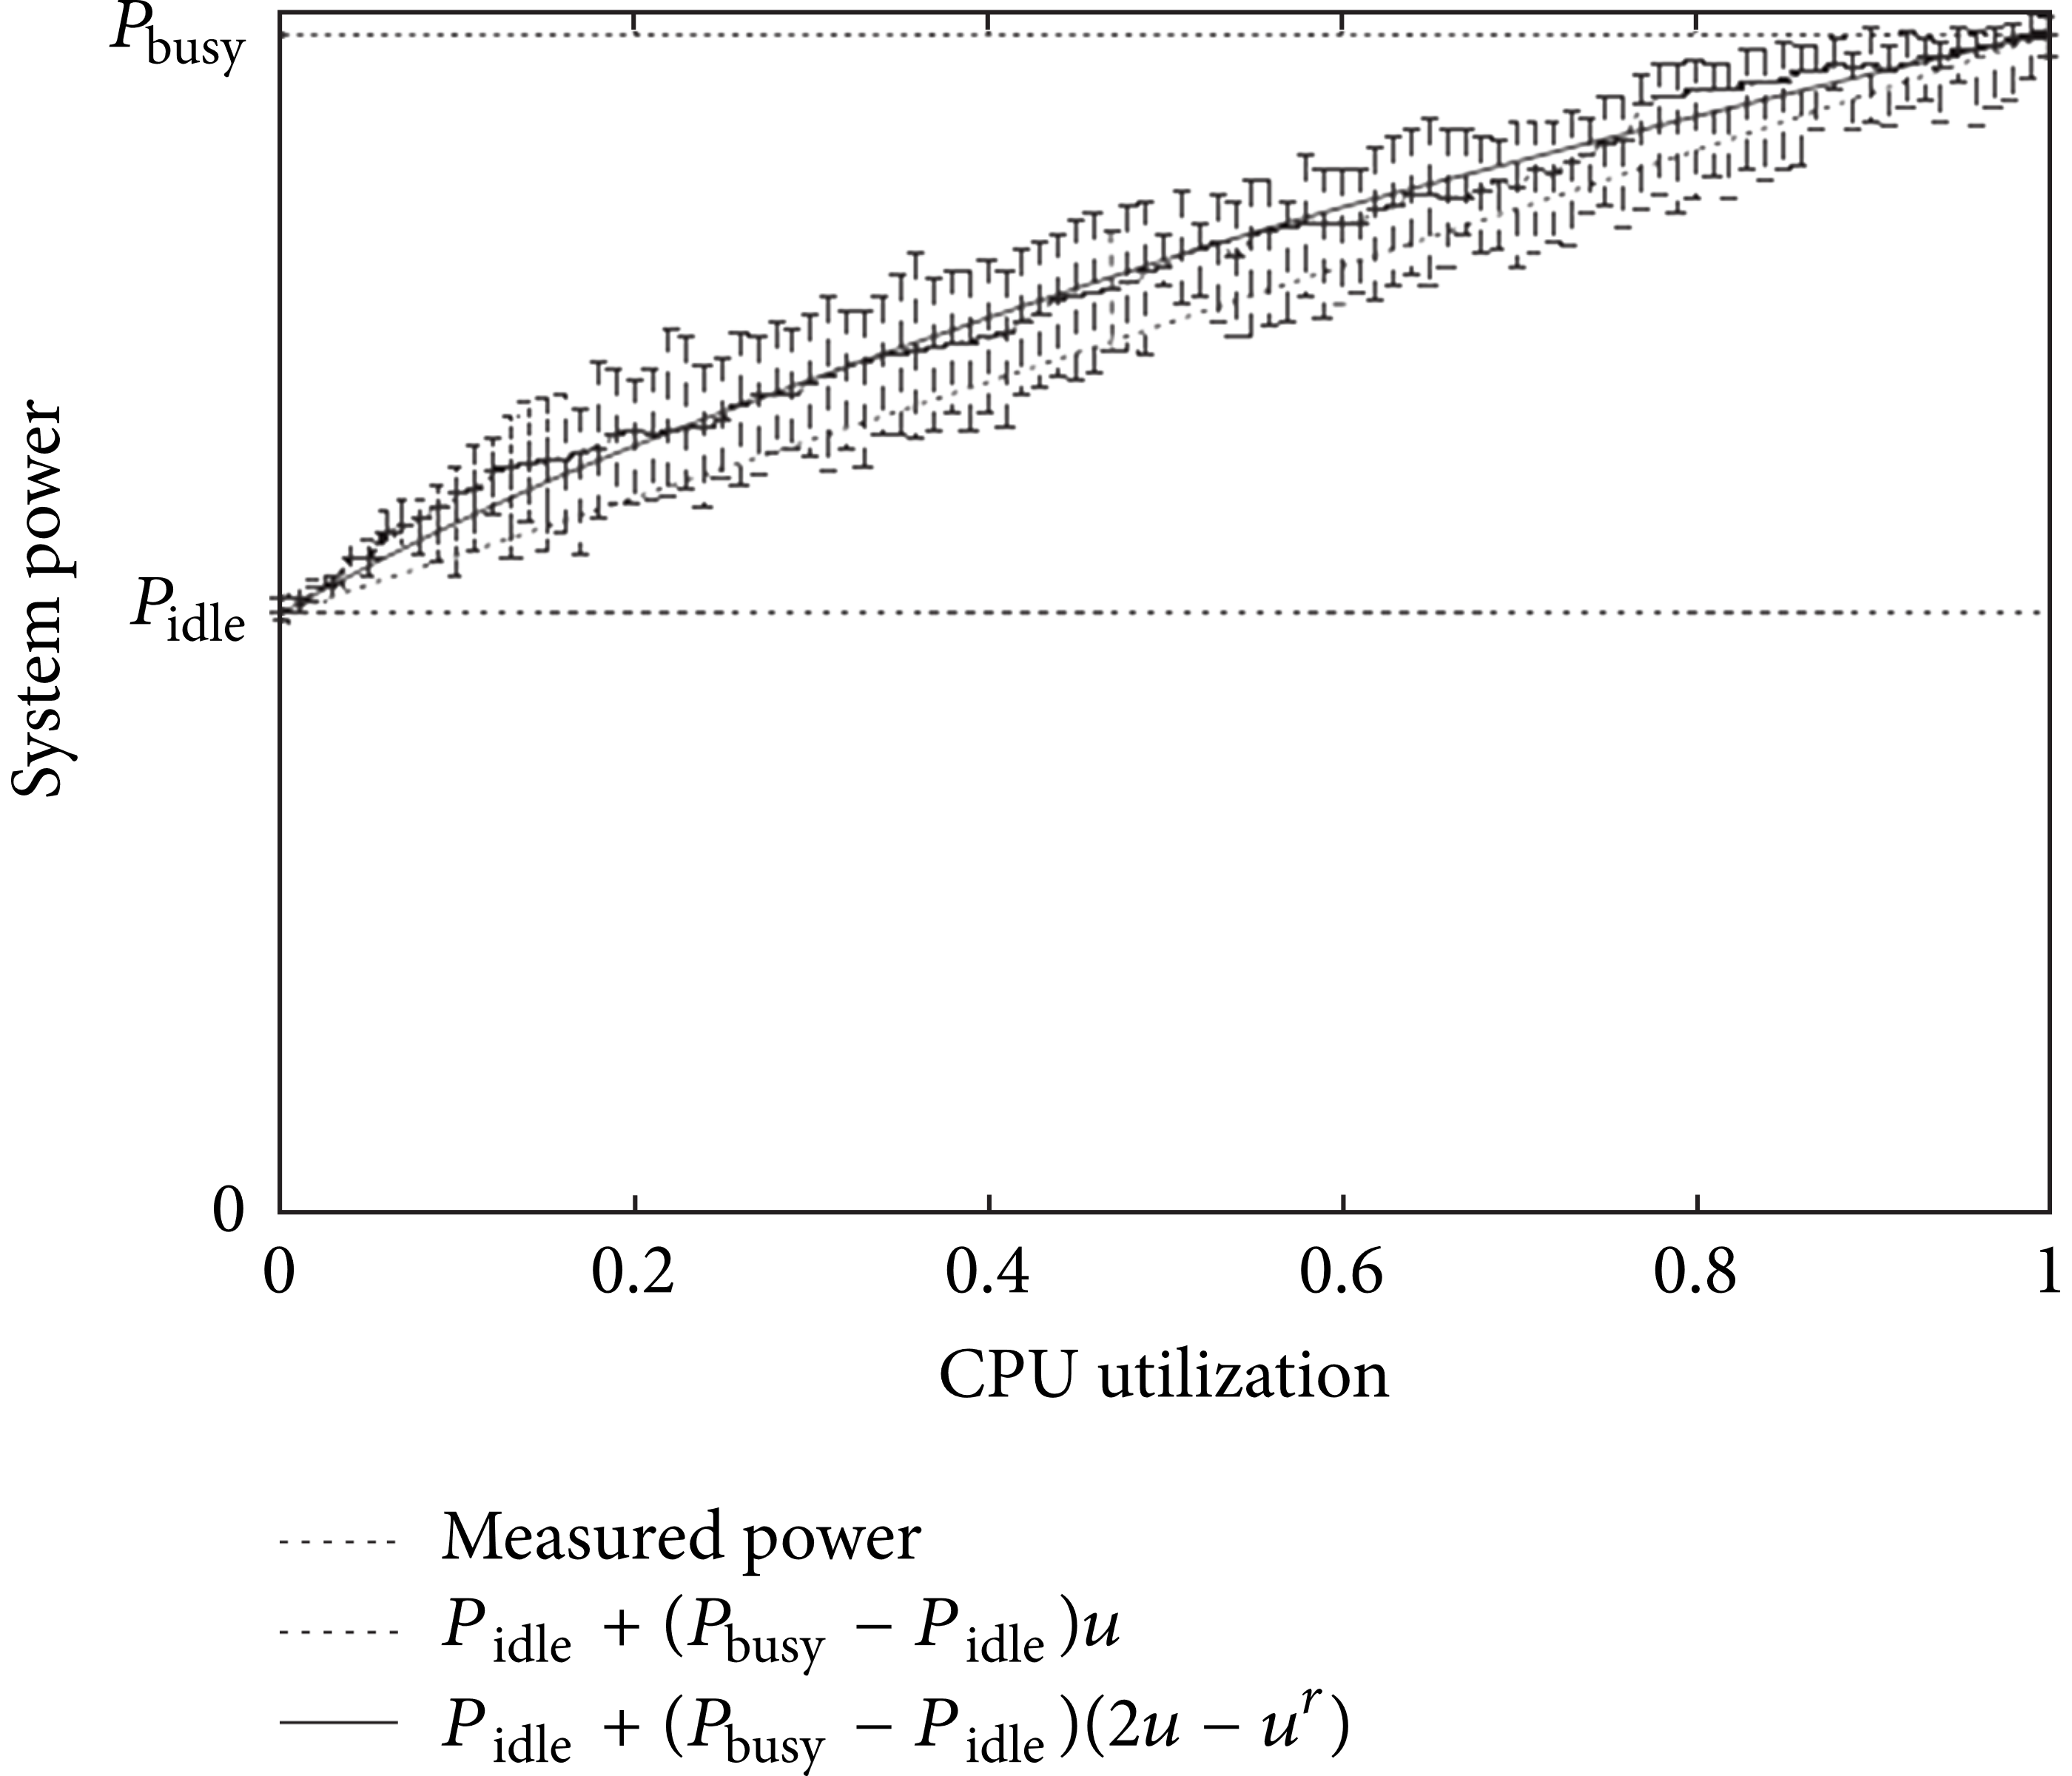
\includegraphics[width=\textwidth]{paper/figures/exempleCPUcurve.png}
      \caption{Exemple de courbe de consommation d'un processeur de serveur \cite{cpuGraph}}
      \label{fig:exempleCPUcurve}
  \end{minipage}
\end{figure}

Ceci fait qu'il est préférable de faire tourner un petit résolveur dns (par exemple pour une entreprise de taille moyenne) sur un plus petit serveur que celui utilisé pour les tests ou encore mieux sur une machine virtuelle afin de partager la consommation avec d'autres applications car plus la machine est utilisé moins elle consomme par cycle cpu "utile".

C'est dans ce genre de cas que des infrastructures telles que Nomad qui déployent les différents services automatiquement en fonction de l'utilisation des différents serveurs peuvent être très efficace.
Il faut cependant tenir compte de la possibilité de pics soudain d'utilisation et de marges de redondance en cas d'échec d'un ou plusieurs serveurs.

\subsection{Nuage Anycast}
Pour ce qui est de la consommation du \gls{anycast}, elle est très constante malgré un volume de requêtes variant du simple au double durant la journée.
\todo{voir pourquoi ?}

\begin{figure}[ht]
  \noindent
  \begin{minipage}{.55\textwidth}
Ici, nous sommes dans une situation demandant beaucoup de redondance et de stabilité dû a l'importance du service fournit (si l'infrastructure ne répond pas, aucun site web ou service en .fr n'est accessible une fois le cache des différent résolveurs expiré)

En conclusion, on rejoins l'idée que la consommation électrique n'est pas directement proportionnelle au nombre de requêtes mais est constante.
(Il faut néanmoins prendre en compte que le volume de requêtes influence le nombre d'équipement réseau et serveur nécessaires mais cette différence n'est présente qu'au niveau macroscopique). \cite{blogStephaneConsoElec}

Il est tout de même intéressant de remarquer qu'une part très importante des requêtes dns envoyés lors d'une session de navigation internet classique est constitué de requêtes liés a la publicité et au traçage (notamment sur les sites de journaux qui peuvent causer des dizaines de requêtes en une seule page). Ce phénomène est aussi visible par le fait que dans le top 10 000 OpenPageRank, il y a 3000+ domaines qui sont des sous-domaines de doubleclick.net, la solution de publicité et de traçage de Google. \cite{openPageRank}
  \end{minipage}
  \hfill
  \begin{minipage}{.40\textwidth}
    \centering
      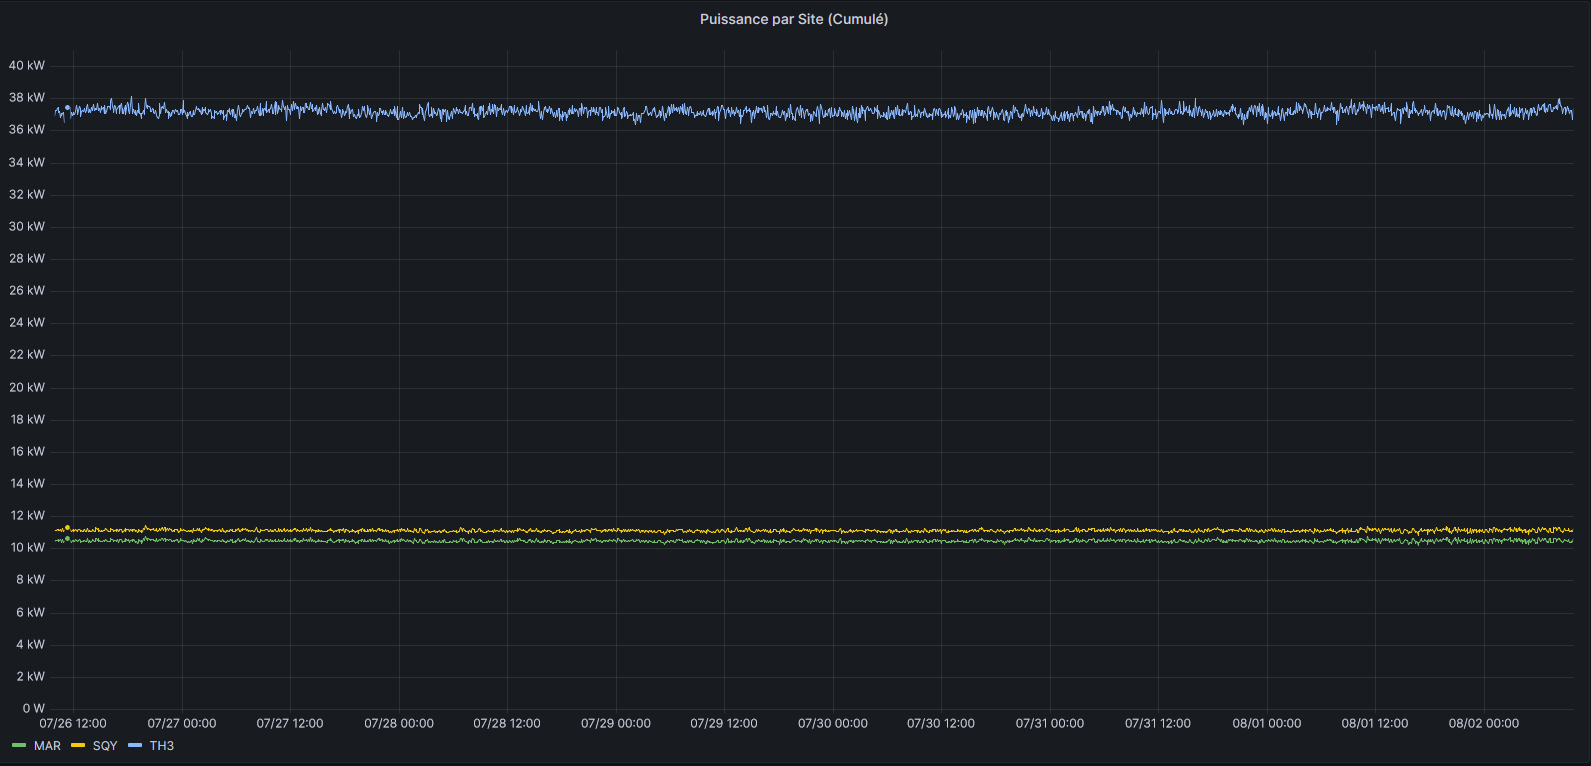
\includegraphics[width=\textwidth]{paper/figures/puissanceParSite.png}
      \caption{Puissance utilisé par site(datacenter)}
      \label{fig:puissanceSite}
  \centering
      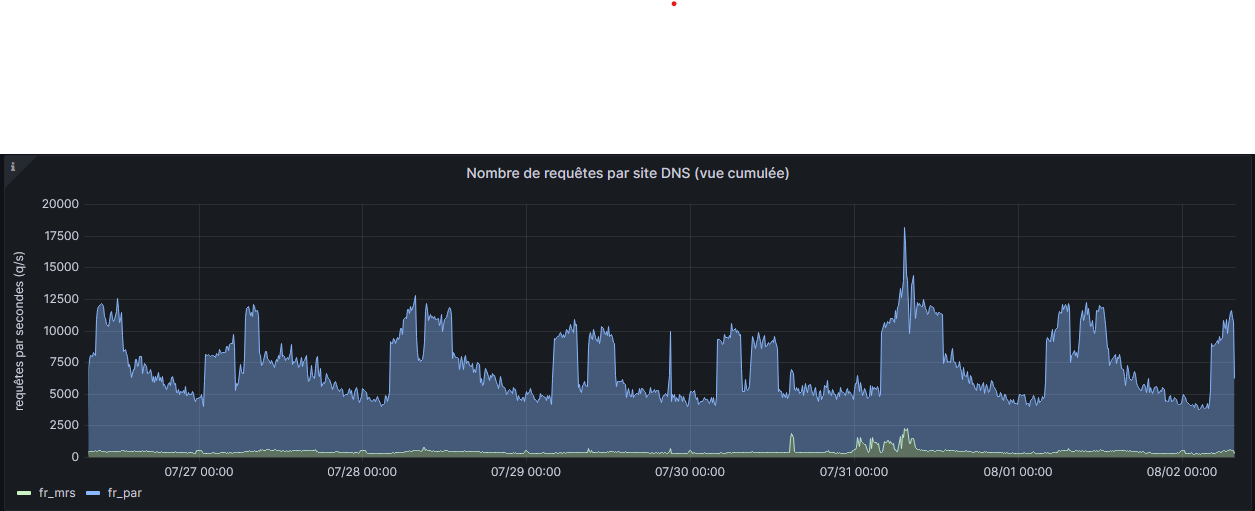
\includegraphics[width=\textwidth]{paper/figures/qpsAnycast.png}
      \caption{Nombre de requêtes par secondes sur le \gls{anycast} de l'afnic}
      \label{fig:QPSAnycast}
  \end{minipage}
\end{figure}

Voir annexe \ref{A:puissanceParSite} et \ref{A:QPSAnycast} pour les graphiques en plus grand